% Cover option D: "millimeter paper" -- the cover looks like a page from a
% problem-solver's notebook: fine graph paper with inked astronomy diagrams
% (a celestial sphere, a Kepler orbit with equal-area sectors).
\documentclass[11pt,a4paper]{article}
\usepackage[margin=0cm]{geometry}
\usepackage[T1]{fontenc}
\usepackage{lmodern}
\usepackage{amsmath}
\usepackage{tikz}
\usetikzlibrary{calc}
\pagestyle{empty}

\definecolor{dpaper}{HTML}{FBF8F1}
\definecolor{dgrid}{HTML}{CFDCE2}
\definecolor{dink}{HTML}{1C2B3A}
\definecolor{dred}{HTML}{BC4B32}

\begin{document}
\begin{tikzpicture}[remember picture,overlay]
  % Paper background.
  \fill[dpaper] (current page.south west) rectangle (current page.north east);

  % Millimeter grid: fine 5 mm lines, stronger 25 mm lines.
  \begin{scope}[shift={(current page.south west)}]
    \foreach \x in {0,0.5,...,21.0}
      \draw[dgrid,opacity=0.45,line width=0.3pt] (\x,0) -- (\x,29.7);
    \foreach \y in {0,0.5,...,29.7}
      \draw[dgrid,opacity=0.45,line width=0.3pt] (0,\y) -- (21,\y);
    \foreach \x in {0,2.5,...,21.0}
      \draw[dgrid,opacity=0.85,line width=0.45pt] (\x,0) -- (\x,29.7);
    \foreach \y in {0.2,2.7,...,29.7}
      \draw[dgrid,opacity=0.85,line width=0.45pt] (0,\y) -- (21,\y);

    % ---------------- celestial sphere sketch, upper right ----------------
    \begin{scope}[shift={(15.3,23.2)}]
      \draw[dink,line width=1.0pt] (0,0) circle (2.9);
      % Equator: front solid, back dashed.
      \draw[dink,line width=0.8pt] (-2.9,0) arc (180:360:2.9 and 0.85);
      \draw[dink,line width=0.6pt,dash pattern=on 2pt off 2pt]
        (2.9,0) arc (0:180:2.9 and 0.85);
      % A meridian.
      \draw[dink,line width=0.8pt] (0,-2.9) arc (270:450:0.85 and 2.9);
      \draw[dink,line width=0.6pt,dash pattern=on 2pt off 2pt]
        (0,2.9) arc (90:270:0.85 and 2.9);
      % Polar axis.
      \draw[dink,line width=0.8pt] (0,-3.5) -- (0,3.5);
      \node[dink,font=\footnotesize\sffamily] at (0.35,3.35) {P};
      % A star with hour-circle arc and declination mark.
      \fill[dred] (37:2.9) circle (2.4pt);
      \draw[dred,line width=0.8pt] (2.9,0) arc (0:37:2.9);
      \node[dred,font=\footnotesize\sffamily] at (22:3.35) {$\delta$};
      \draw[dred,line width=0.7pt,-stealth] (0,0) -- (37:2.82);
    \end{scope}

    % ---------------- Kepler orbit sketch, lower half ----------------
    \begin{scope}[shift={(12.6,6.4)}]
      \draw[dink,line width=1.0pt] (0,0) ellipse (5.1 and 3.2);
      % Sun at the focus (c = sqrt(a^2-b^2) = 3.97).
      \fill[dred] (3.97,0) circle (4.2pt);
      \foreach \a in {0,45,...,315}
        \draw[dred,line width=0.6pt]
          ($(3.97,0)+(\a:0.32)$) -- ($(3.97,0)+(\a:0.48)$);
      % Fast sector near perihelion.
      \fill[dred,opacity=0.28]
        (3.97,0) -- plot[domain=8:38,samples=24]
          ({5.1*cos(\x)},{3.2*sin(\x)}) -- cycle;
      % Slow sector near aphelion: equal area, wider arc.
      \fill[dred,opacity=0.28]
        (3.97,0) -- plot[domain=143:172,samples=24]
          ({5.1*cos(\x)},{3.2*sin(\x)}) -- cycle;
      % Radius vector and true anomaly, both anchored at the focus.
      \draw[dink,line width=0.8pt,-stealth]
        (3.97,0) -- ({5.1*cos(110)},{3.2*sin(110)});
      \node[dink,font=\footnotesize\sffamily] at (0.7,1.95) {$r$};
      \draw[dink,line width=0.7pt] (4.87,0) arc (0:152:0.9);
      \node[dink,font=\footnotesize\sffamily] at (4.55,1.25) {$\theta$};
      % Apside line.
      \draw[dink,line width=0.5pt,dash pattern=on 2pt off 2pt]
        (-5.5,0) -- (5.5,0);
      \node[dink,font=\footnotesize\sffamily\itshape,align=left]
        at (2.1,-3.95) {equal areas in equal times};
    \end{scope}

    % A small inked annotation formula, mid-page right.
    \node[dink,font=\normalsize,anchor=west] at (12.9,12.4)
      {$\dfrac{T^2}{a^3}=\dfrac{4\pi^2}{GM}$};
  \end{scope}

  % ---------------- title block, left ----------------
  \begin{scope}[shift={(current page.north west)}]
    \node[anchor=west,dink,font=\small\sffamily\scshape] at (2.2,-3.1)
      {International Olympiad on Astronomy \& Astrophysics};
    \draw[dred,line width=1.6pt] (2.24,-3.75) -- (7.0,-3.75);
    \node[anchor=west,dink,font=\fontsize{40}{44}\selectfont\sffamily\bfseries]
      at (2.15,-5.4) {IOAA};
    \node[anchor=west,dink,font=\fontsize{40}{44}\selectfont\sffamily\bfseries]
      at (2.15,-7.0) {Problem Book};
    \node[anchor=west,dink,font=\large\sffamily,align=left] at (2.2,-9.4)
      {Problems and available official solutions\\ organized by topic};
    \node[anchor=west,dred,font=\LARGE\sffamily\bfseries] at (2.2,-11.4)
      {2007--2025};
  \end{scope}
  \node[anchor=west,dink,font=\normalsize\sffamily]
    at ($(current page.south west)+(2.2,2.0)$)
    {Compiled and edited by Ioana A.~Zelko};
\end{tikzpicture}
\end{document}
